\section{Algorithm}
The algorithm is structured in three sequential steps, which we will discuss in more detail in the following subsections.

%The first step is to generate a hypergraph based on the main goal (what the exercise asks us to prove) and the target goal (the part of the student's proof we want to complete), in order to store all possible rule applications for both goals. Then, we use this graph to build a second hypergraph that simulates as many proof constructions as possible by decomposing the target goal into sub-goals. In the last step, we trim this second graph so that it retains only valid and minimal proofs, either in terms of the number of steps required or the height needed to solve the problem. Finally, we use the resulting graph to extract and build readable proofs, which can later be used to generate feedback.

\subsection{Transition Graph}
The first step is to create the Transition Graph (TG). This graph stores the formulas that might be part of the final proof, as well as the rules that can be applied to each formula. In short, the TG sets up the rules of the "game".

To generate the graph, we need to specify the main goal of the exercise \(\Gamma \vdash \varphi\), what the exercise wants us to prove, and the target goal \(\Sigma \vdash \theta\), which is the part of the proof that needs to be completed. The main goal is used to generate all the natural proof paths, which are proofs built using only formulas derived from decomposing the main goal. The target goal, on the other hand, can sometimes be used to generate non-natural proof paths. By this, we mean proofs that include more complex formulas than those directly derived from the main goal. By considering both goals, the system is able to generate more personalized and user-guided proofs, as it also takes into account the deviations made by the user, which is one of the core elements of our algorithm.

Before we describe the procedure, let us introduce some definitions:
\begin{definition}[Labeled Directed Hypergraph with Labeled Heads]
A \emph{Labeled Directed Hypergraph with Labeled Heads} is a pair
\[
H = (V, E),
\]
where:
\begin{itemize}
  \item \( V \) is a finite set of \emph{nodes}, and
  \item \( E \subseteq V \times \mathcal{P}(V \times (V \cup \{\varepsilon\})) \times L \) is a finite set of \emph{labeled hyperedges}, where each hyperedge consists of:
  \begin{itemize}
    \item a \emph{tail}, which is a single input node from \( V \),
    \item a \emph{labeled head}, which is a set of pairs \( (v, w) \in V \times (V \cup \{\varepsilon\}) \), where \( v \) is a head node and \( w \) is either a node or the empty symbol \( \varepsilon \), and
    \item a label \( \ell \in L \).
  \end{itemize}
\end{itemize}
\end{definition}

\begin{definition}[Transition Graph]
A \emph{Transition Graph (TG)} is a pair
\[
T_G = (F, T_E),
\]
where:
\begin{itemize}
  \item \( F \) is a finite set of \emph{formulas}, and
  \item \( T_E \subseteq F \times \mathcal{P}(F \times (F \cup \{\varepsilon\})) \times R \) is a finite set of \emph{labeled hyperedges} called \emph{Transition Edge (TE)}, where each edge consists of:
  \begin{itemize}
    \item a tail formula \( f \in F \),
    \item a set of pairs \( (f_1, f_2) \in F \times (F \cup \{\varepsilon\}) \), where \( f_1 \) is a \emph{hypothesis} and \( f_2 \) is a \emph{closed hypothesis}, and
    \item a rule \( r \in R \).
  \end{itemize}
\end{itemize}
\end{definition}

A TE is the application of a rule to a formula. Figure \ref{fig:te-ex} shows an example of the rule being applied \(\vee_E\) and the corresponding edge.

    \begin{figure}
        \centering
        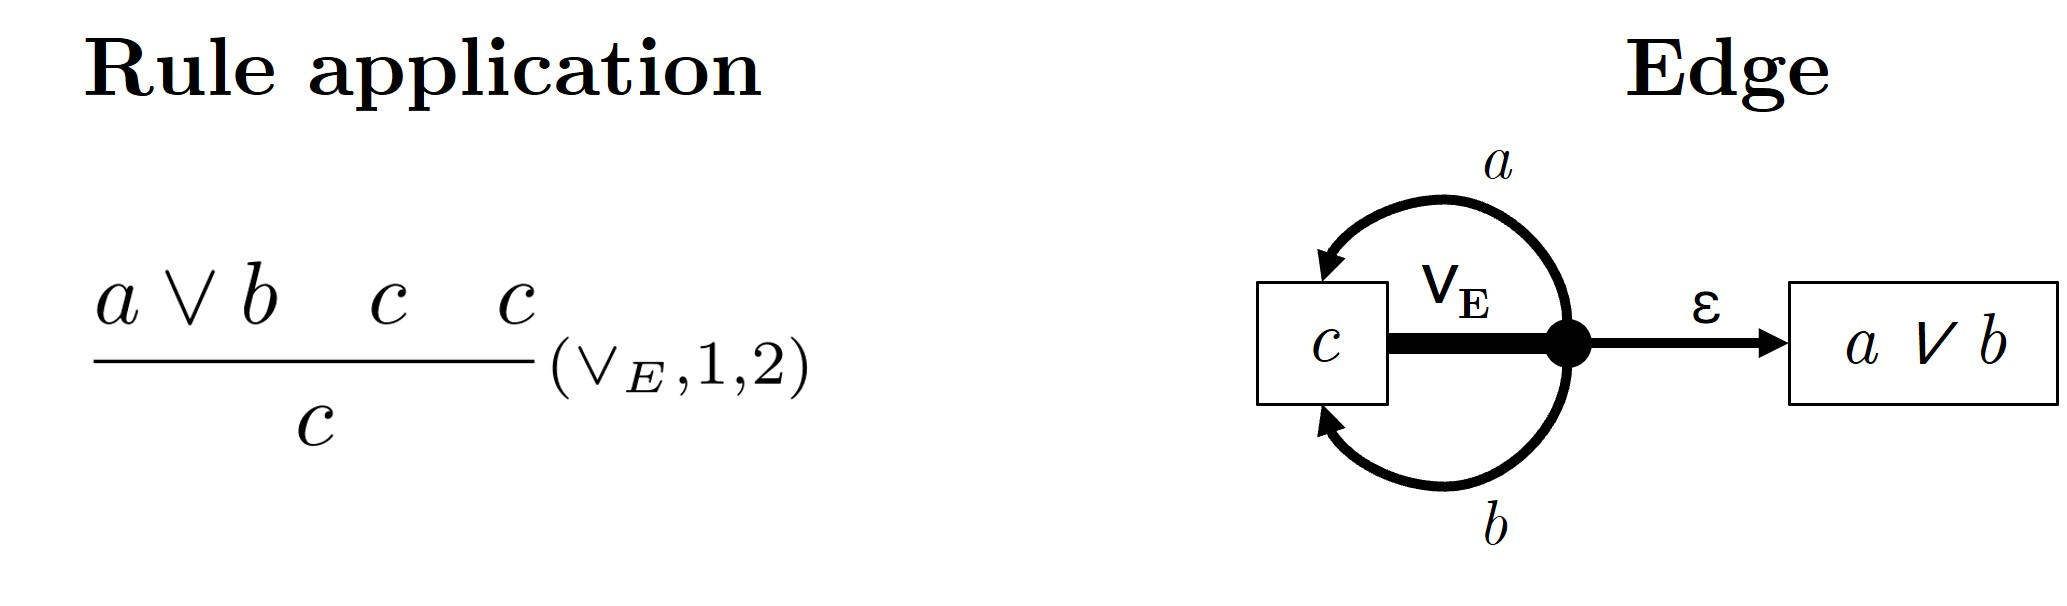
\includegraphics[width=0.8\linewidth]{resources/te-example.jpg}
        \caption{Example of a transition edge.}
        \label{fig:te-ex}
    \end{figure}

We will have \(T_E = T_E \cup \{(c, \{(a \vee b, \varepsilon), (c, a), (c, b)\}, \vee_E)\}\). Our edges always point from the conclusion to its hypotheses. If we were working with FOL proofs, we would also need to consider side conditions as part of T. The reason for using this type of graph is that it allows us to map rule applications directly into a data structure. In the final step, we will explain why it is necessary to store edges in this way. At this point, there is no need to keep track of the marks, since they can be easily added in the final steps when reconstructing the full proof.

\vspace{1em}
With all the necessary definitions in place, we now present the procedure to generate the TG, as shown in Algorithm~\ref{alg:tg-construction}.

\begin{algorithm}
\caption{Transition Graph Construction}
\label{alg:tg-construction}
\KwIn{Main goal $\Gamma \vdash \varphi$, Target goal $\Sigma \vdash \theta$}
\KwOut{Transition Graph $T_G = (F, T_E)$}

$F \leftarrow \Gamma \cup \Sigma \cup \{\varphi, \theta\}$ \tcp*[r]{Initialize formulas}
$T_E \leftarrow \emptyset$ \tcp*[r]{Initialize edges}

\tcp{Compute formulas}
\ForEach{$f \in F$}{
  \If{$f $was not already added as a negation}{
    $F \leftarrow F \cup \{\lnot f\}$ \tcp*[r]{Add negation for indirect rules}
  }

  Decompose $f$ into parts $S$\;
  $F \leftarrow F \cup S$\;
}

\tcp{Compute transitions}
\ForEach{$f \in F$}{
    
    \If{$f$ was not added as a negation}{
        $T_E = T_E \cup \{(f, \{(\bot, \lnot f)\}, \bot)\}$\;
    }

    \If{$f = \lnot \alpha$ for some $\alpha$}{
        $T_E = T_E \cup \{(\lnot \alpha, \{(\bot, \alpha)\}, \lnot_I)\}$\;
        $T_E = T_E \cup \{(\bot, \{(\alpha, \varepsilon), (\lnot \alpha,\varepsilon)\}, \lnot_E)\}$\;
    }

    \If{$f = \alpha \lor \beta$ for some $\alpha, \beta$}{
        $T_E = T_E \cup \{(f, \{(\alpha, \varepsilon)\}, \vee_{I_R})\}$\;
        $T_E = T_E \cup \{(f, \{(\beta, \varepsilon)\}, \vee_{I_L})\}$\;
        \ForEach{$f' \in F$}{
            $T_E = T_E \cup \{(f', \{(f, \varepsilon), (f',\alpha), (f', \beta)\}), \vee_E\}$\;
        }
    }

    \If{$f = \alpha \land \beta$ for some $\alpha, \beta$}{
        $T_E = T_E \cup \{(\alpha \land \beta, \{(\alpha, \varepsilon), (\lnot \beta,\varepsilon)\}, \land_{I})\}$\;
        $T_E = T_E \cup \{(\alpha, \{(\alpha \land \beta, \varepsilon)\}, \land_{E_R})\}$\;
        $T_E = T_E \cup \{(\beta, \{(\alpha \land \beta, \varepsilon)\}, \land_{E_L})\}$\;
    }

    \If{$f = \alpha \to \beta$ for some $\alpha, \beta$}{
        $T_E = T_E \cup \{(\alpha \to \beta, \{(\beta, \alpha)\}, \to_{I})\}$\;
        $T_E = T_E \cup \{(\beta, \{(\alpha, \varepsilon), (\alpha \to \beta, \varepsilon)\}, \to_{E})\}$\;
    }

}

\end{algorithm}

The computing of formulas and transitions can be done in one step to avoid unnecessary loops, but for simplicity, we kept them separate. The decomposing step is an important part to know in advance which formulas we will have in the graph and also to match with formulas that require that information, since they can be applied to every formula, such as the Elimination of Disjunction rule. The decomposition is done by splitting the formula at the outermost logical operators (if it is not an atomic formula). For example, $a \to \lnot b$ can be split into $a$ and $\lnot b$, but $a$ cannot be decomposed since it is atomic. However, we can decompose $\lnot b$ into just $b$.

To illustrate the construction process in detail, we now present a full example in Figure~\ref{fig:tg-final}, based on the specific main goal and target goal \(\vdash a \to a\) (so we want a full proof for the problem).

\begin{figure}
    \centering
    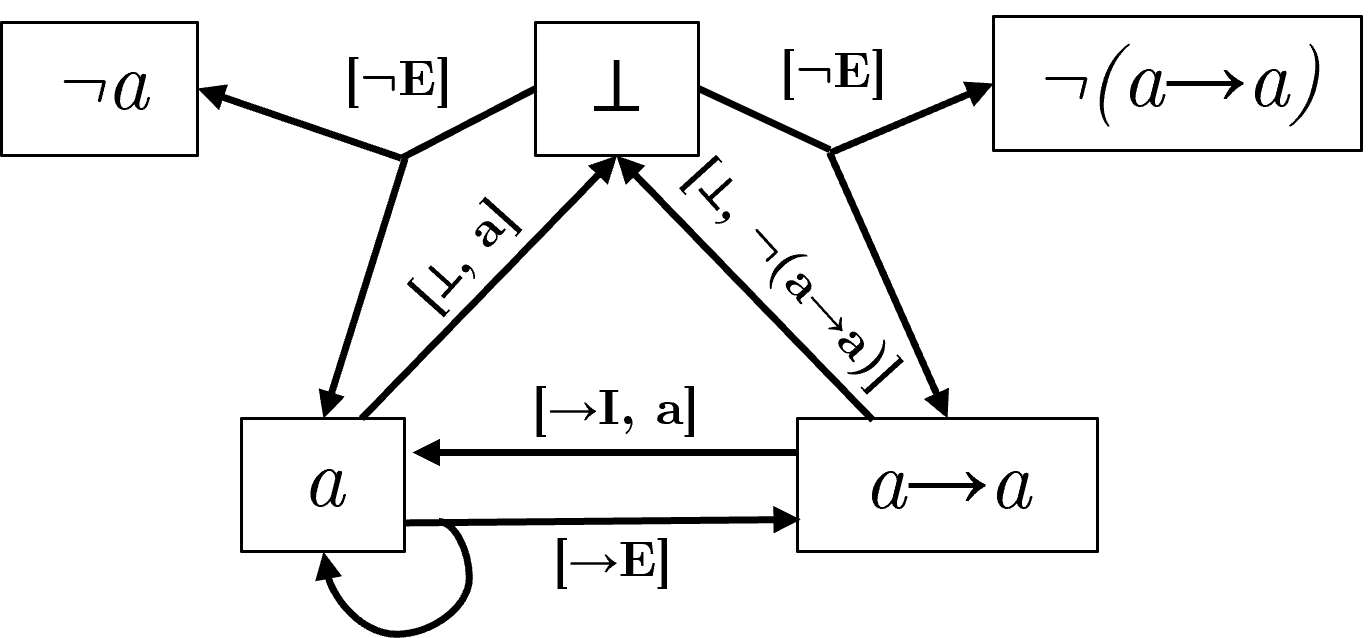
\includegraphics[width=1\linewidth]{resources/tg-final.png}
    \caption{Final TG generated from main goal and target goal \(\vdash a \to a\)}
    \label{fig:tg-final}
\end{figure}

\subsection{Proof Graph}
The second step is to build the Proof Graph (PG). The structure of this graph is very similar to the TG, but it stores different objects. It stores the possible sub-goals derived from the target goal. In this graph, the nodes are goals, and the edges are adaptations of transition edges (TE) that now store goals. The purpose of this graph is to decompose the target goal into smaller goals that are easier to prove, until we reach goals that can be directly proved. In the end, after generating all sub-goals, the graph may contain multiple proof paths. Some of these paths may not lead to a solution, while others may succeed in proving the target goal.

To generate the PG, we use the TG, previously generated, and the target goal. Note that the target goal can also be the initial goal, in case we want to generate a full proof for the problem. Before we describe the procedure, we define some key terms:

\begin{definition}[Proof Graph]
A \emph{Proof Graph (PG)} is a pair
\[
P_G = (G, P_E),
\]
where:
\begin{itemize}
  \item \( FG \) is a finite set of \emph{goals}, and
  \item \( P_E \subseteq G \times \mathcal{P}(G \times (F \cup \{\varepsilon\})) \times R \) is a finite set of \emph{labeled hyperedges} called \emph{Proof Edge (PE)}, where each edge consists of:
  \begin{itemize}
    \item a tail goal \( g \in G \),
    \item a set of pairs \( (g_1, f_1) \in G \times (F \cup \{\varepsilon\}) \), where \( g_1 \) is a goal and \( f_1 \) is a \emph{closed hypothesis}, and
    \item a rule \( r \in R \).
  \end{itemize}
\end{itemize}
\end{definition}

\begin{definition}[Proved Goal]
A goal \( \Delta \vdash \delta \) is \emph{proved} if either:
\begin{itemize}
  \item \( \delta \in \Delta \), or
  \item there exists a Proof Edge \( (g, T, r) \in P_E \) in the Proof Graph \( P_G = (G, P_E) \), such that \( g = \Delta \vdash \delta \), and for every pair \( (g_1, f_1) \in T \), the goal \( g_1 \) is proved.
\end{itemize}
\end{definition}

The definition of proved goal is extremely important because it is used as a stopping condition to avoid the algorithm looping through unnecessary goals and to guarantee that the proof is valid. This is only possible due to the type of graph chosen, as it allows us to capture the relation between the hypotheses and the conclusion of each rule application. Figure~\ref{fig:pe-ex} shows an example of a PE and how these relations can be captured. In the figure, we want to prove \(\{a \vee b\} \vdash a\). By applying the Elimination of Disjunction rule, we notice that one of the hypotheses cannot be closed using only this rule, even if the other two hypotheses are closed. So, what we actually prove with this rule is \(\{a \vee b, a\} \vdash a\), which is different from our goal. To accurately track which goals are proved and ensure the proof only contains valid proved goals, this information must be stored in a hypergraph structure. This is why hypergraphs are necessary.

\begin{figure}
    \centering
    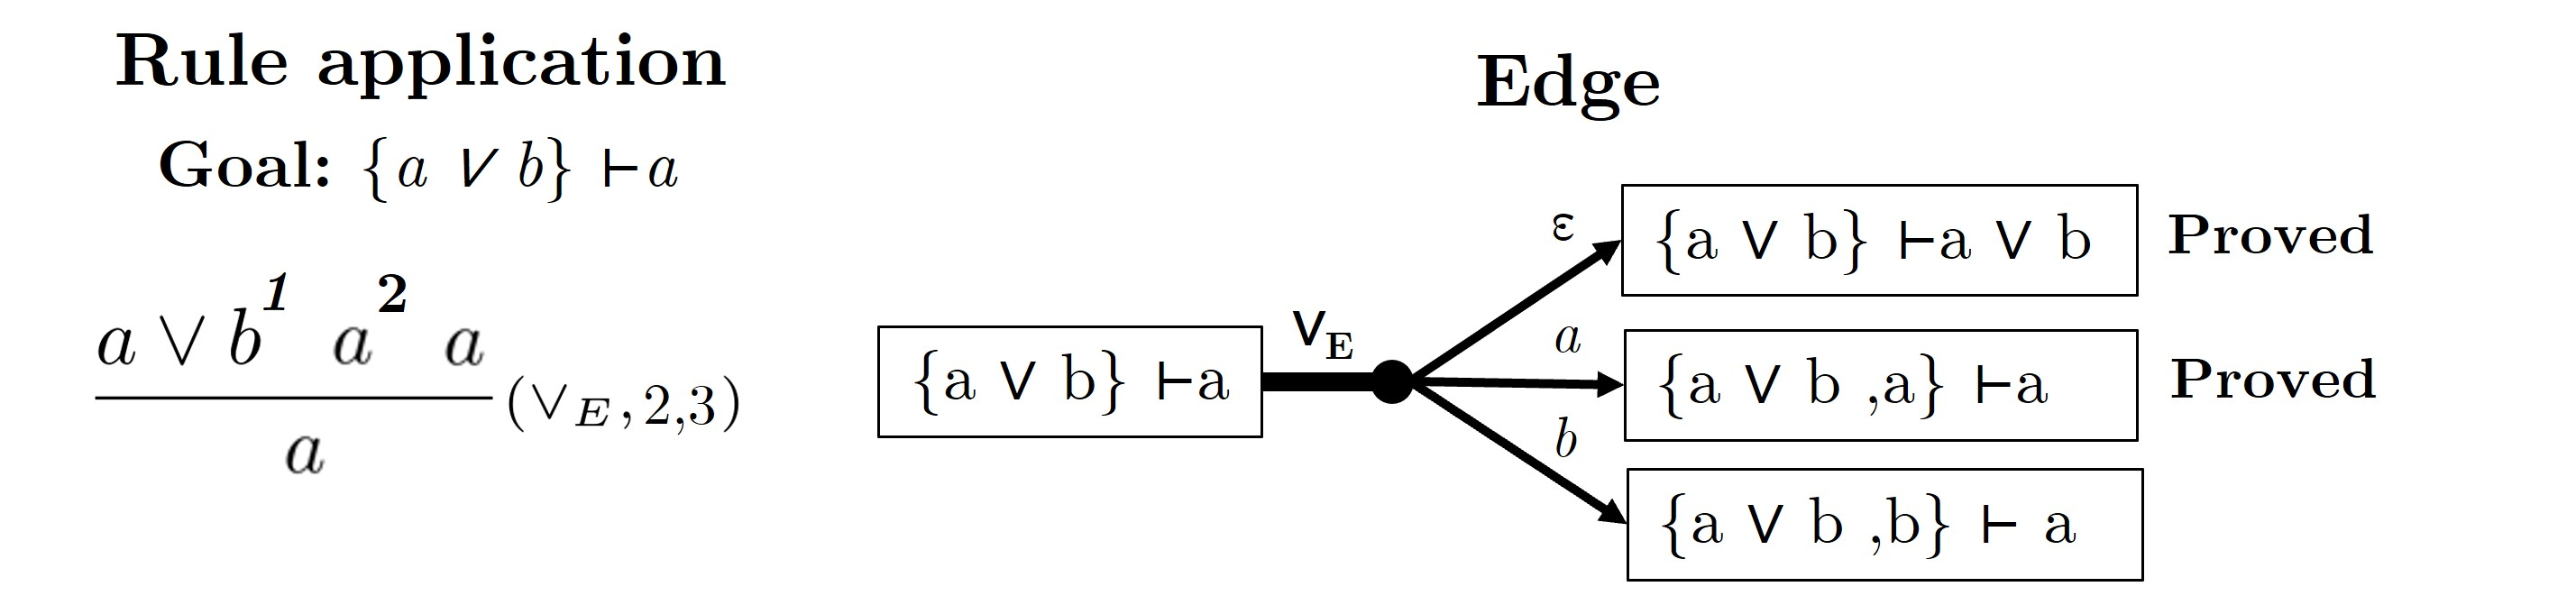
\includegraphics[width=1\linewidth]{resources/pe-example.jpg}
    \caption{Prove \(\{a \vee b\} \vdash a\) using the Elimination of Disjunction rule}
    \label{fig:pe-ex}
\end{figure}

\vspace{1em}
With all the necessary definitions in place, we now present the procedure to generate the PG, as shown in Algorithm~\ref{alg:pg-construction}.

\begin{algorithm}
\caption{Proof Graph Construction}
\label{alg:pg-construction}
\KwIn{Transition Graph $T_G = (F, T_E)$, Target goal $t_g$}
\KwOut{Proof Graph $P_G = (G, P_E)$}

$G \leftarrow \{t_g\}$ \tcp*[r]{Initialize set of goals}
$P_E \leftarrow \emptyset$ \tcp*[r]{Initialize set of proof edges}

\tcp{Compute sub-goals}
\ForEach{$g = \Sigma \vdash \theta \in G$}{

    \If{$g$ is proved}{
        \textbf{continue} \tcp*[r]{Skip proved goal}
    }

    \If{stopping condition is reached}{
        \textbf{break} \tcp*[r]{Avoid excessive expansion}
    }

    \tcp{Get transition edges for formula $\theta$}
    $TE_\theta \leftarrow \{ (f, H, r) \in T_E \mid f = \theta \}$\;

    \ForEach{$(f, H, r) \in TE_\theta$}{
        $T \leftarrow \emptyset$  \tcp*[r]{Store transitions to each hypothesis}
        
        \ForEach{$(f_1, f_2) \in H$}{
            \tcp{Create sub-goal by extending the current premises with the closed hypothesis}
            $g_\text{new} \leftarrow (\Sigma \cup \{f_2\}) \vdash f_1$\;

            $T \leftarrow T \cup \{(g_\text{new}, f_2)\}$\;
            $G \leftarrow G \cup \{g_\text{new}\}$ \tcp*[r]{Add sub-goal}
        }

        $P_E \leftarrow P_E \cup \{(g, T, r)\}$ \tcp*[r]{Add proof edge}
    }
}
\end{algorithm}

This part of the algorithm can generate very large graphs, potentially exponential in size, with millions of distinct goals depending on the complexity of the problem. In most cases, we do not want to explore the entire goal space, as many goals are extremely complex and do not provide useful feedback. Therefore, stopping conditions are required. These may include: limiting the total number of goals explored, setting a maximum number of hypotheses allowed per goal, or enforcing a timeout.

Figure~\ref{fig:st-ex} shows the PG generated using the TG from Figure~\ref{fig:tg-final} and target goal \(\vdash a \to a\), with a limit of 9 goals explored. Nodes with solid borders represent proved goals, while nodes with dashed borders represent unproved goals. Since our target goal is proved, we know that at least one solution was found.

\begin{figure}
    \centering
    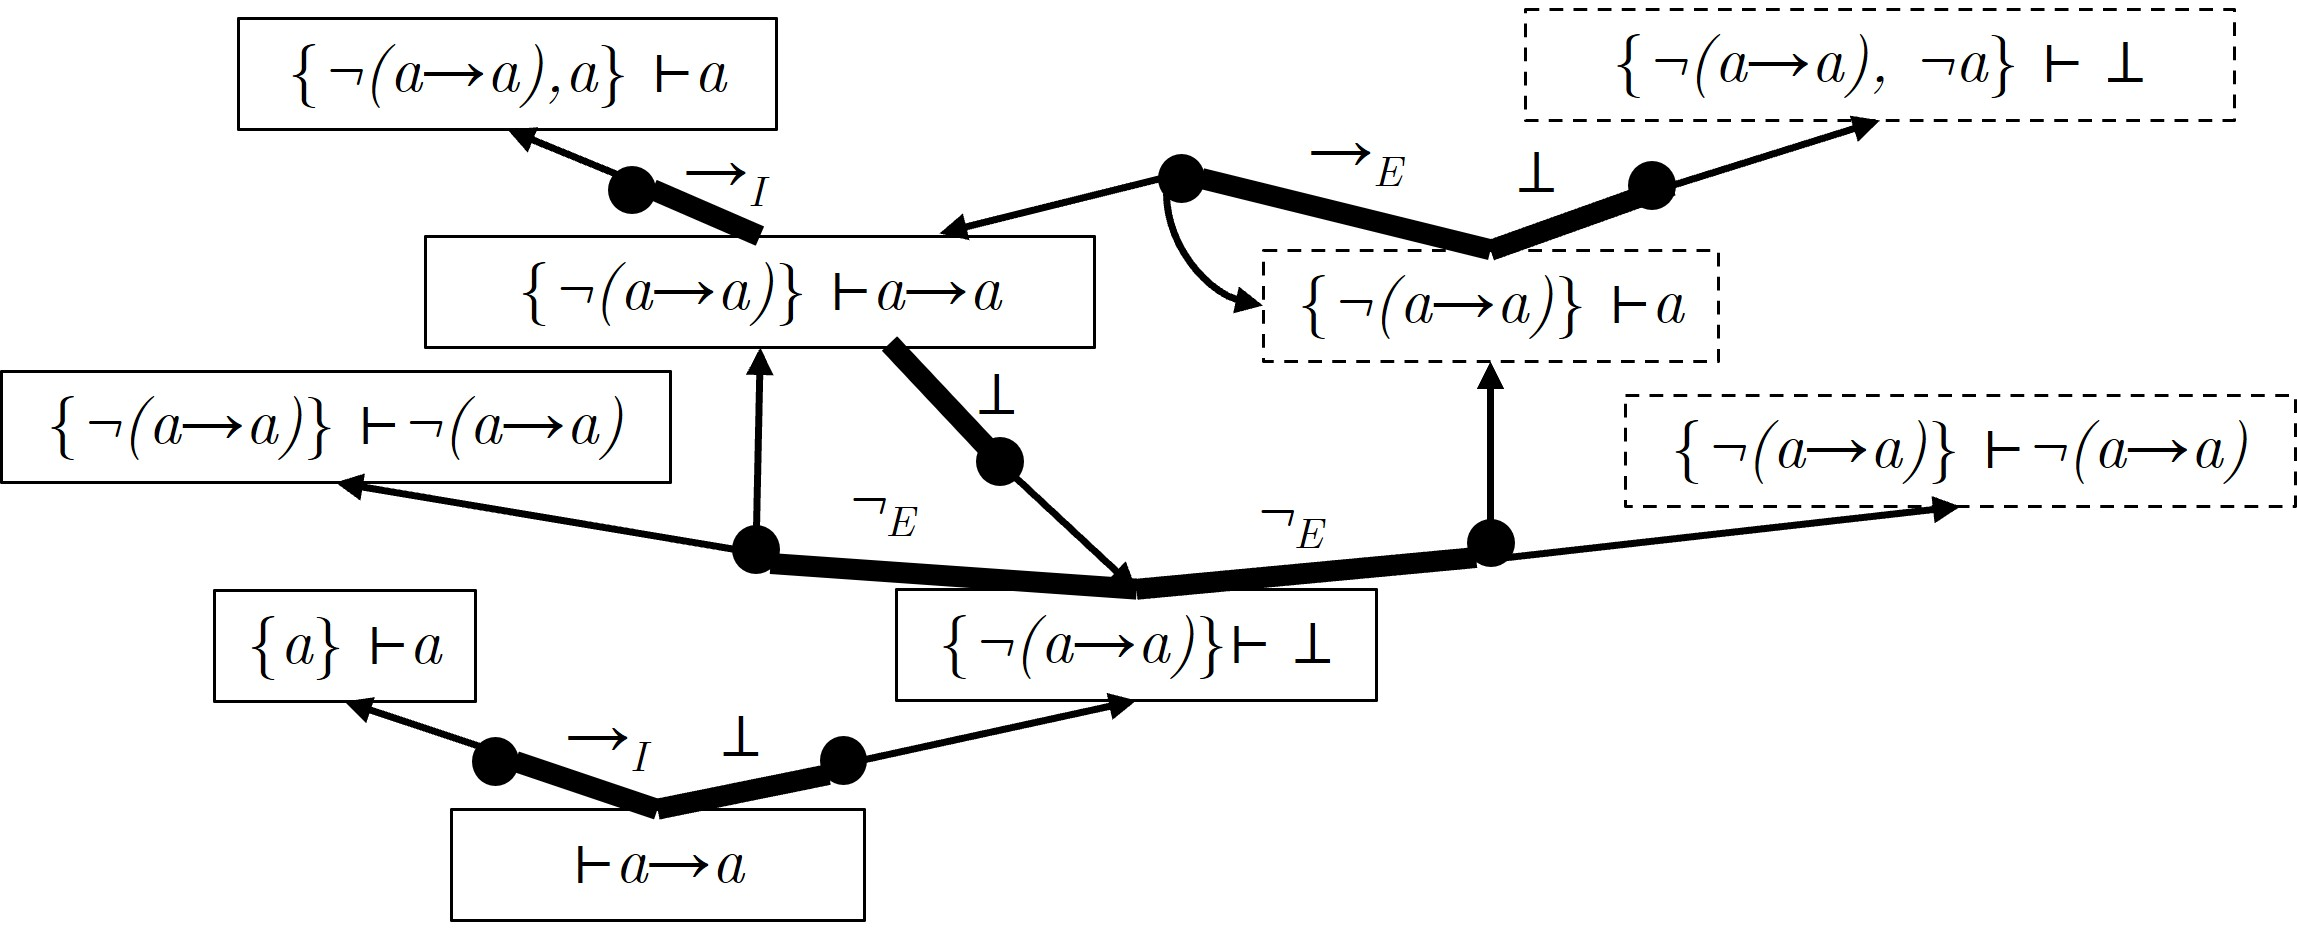
\includegraphics[width=1\linewidth]{resources/sg-gen.jpg}
    \caption{Example of Proof Graph using the TG from Figure~\ref{fig:tg-final} and target goal \(\vdash a \to a\)}
    \label{fig:st-ex}
\end{figure}



\subsection{Trim Graph}

The final stage of our algorithm is to trim the SG and keep only the valid solutions to the problem. In other words, the final trimmed graph will contain only states that lead to a complete and valid proof. To achieve this, we remove unclosed states and extra edges from the SG.

We define two different strategies to trim the graph. Both use a standard graph traversal technique, breadth-first search, to identify which states and edges should be kept. The difference lies in what each strategy prioritizes: the \textbf{Height Trim Strategy} focuses on finding proofs with the smallest height (fewest layers of rule applications), while the \textbf{Size Trim Strategy} aims to find proofs with the fewest total steps (smallest number of rule applications).


\vspace{1em}
\textbf{Height Trim Strategy Procedure:}  
This strategy loops through all closed states and tracks the height needed to reach each one. For every descendant of a closed state, the algorithm continues this tracking process. Because it uses breadth-first traversal, the first time a node is reached, it’s guaranteed to be through the shortest possible path (in terms of height). This makes the strategy efficient.

\vspace{0.5em}
\textbf{Size Trim Strategy Procedure:}  
This strategy also starts from closed states. It updates the size (number of steps) required to reach each ancestor. For each state, it keeps only the edge that leads to a smaller proof. For every descendant
of a closed state, the algorithm continues this tracking process. This process ensures that each state keeps at most one optimal incoming edge, leading to the shortest proof found within the SG's search space. Although slower than the height trim strategy, it finds more concise proofs in terms of rule applications.

\vspace{1em}
Figure~\ref{fig:sg-trim} shows an example of a trimmed SG using the \textbf{Size Trim Strategy}, on the SG shown in Figure~\ref{fig:st-ex}. The states that could not be closed were removed, and the edges coming from higher-level solutions were also trimmed.

\begin{figure}
    \centering
    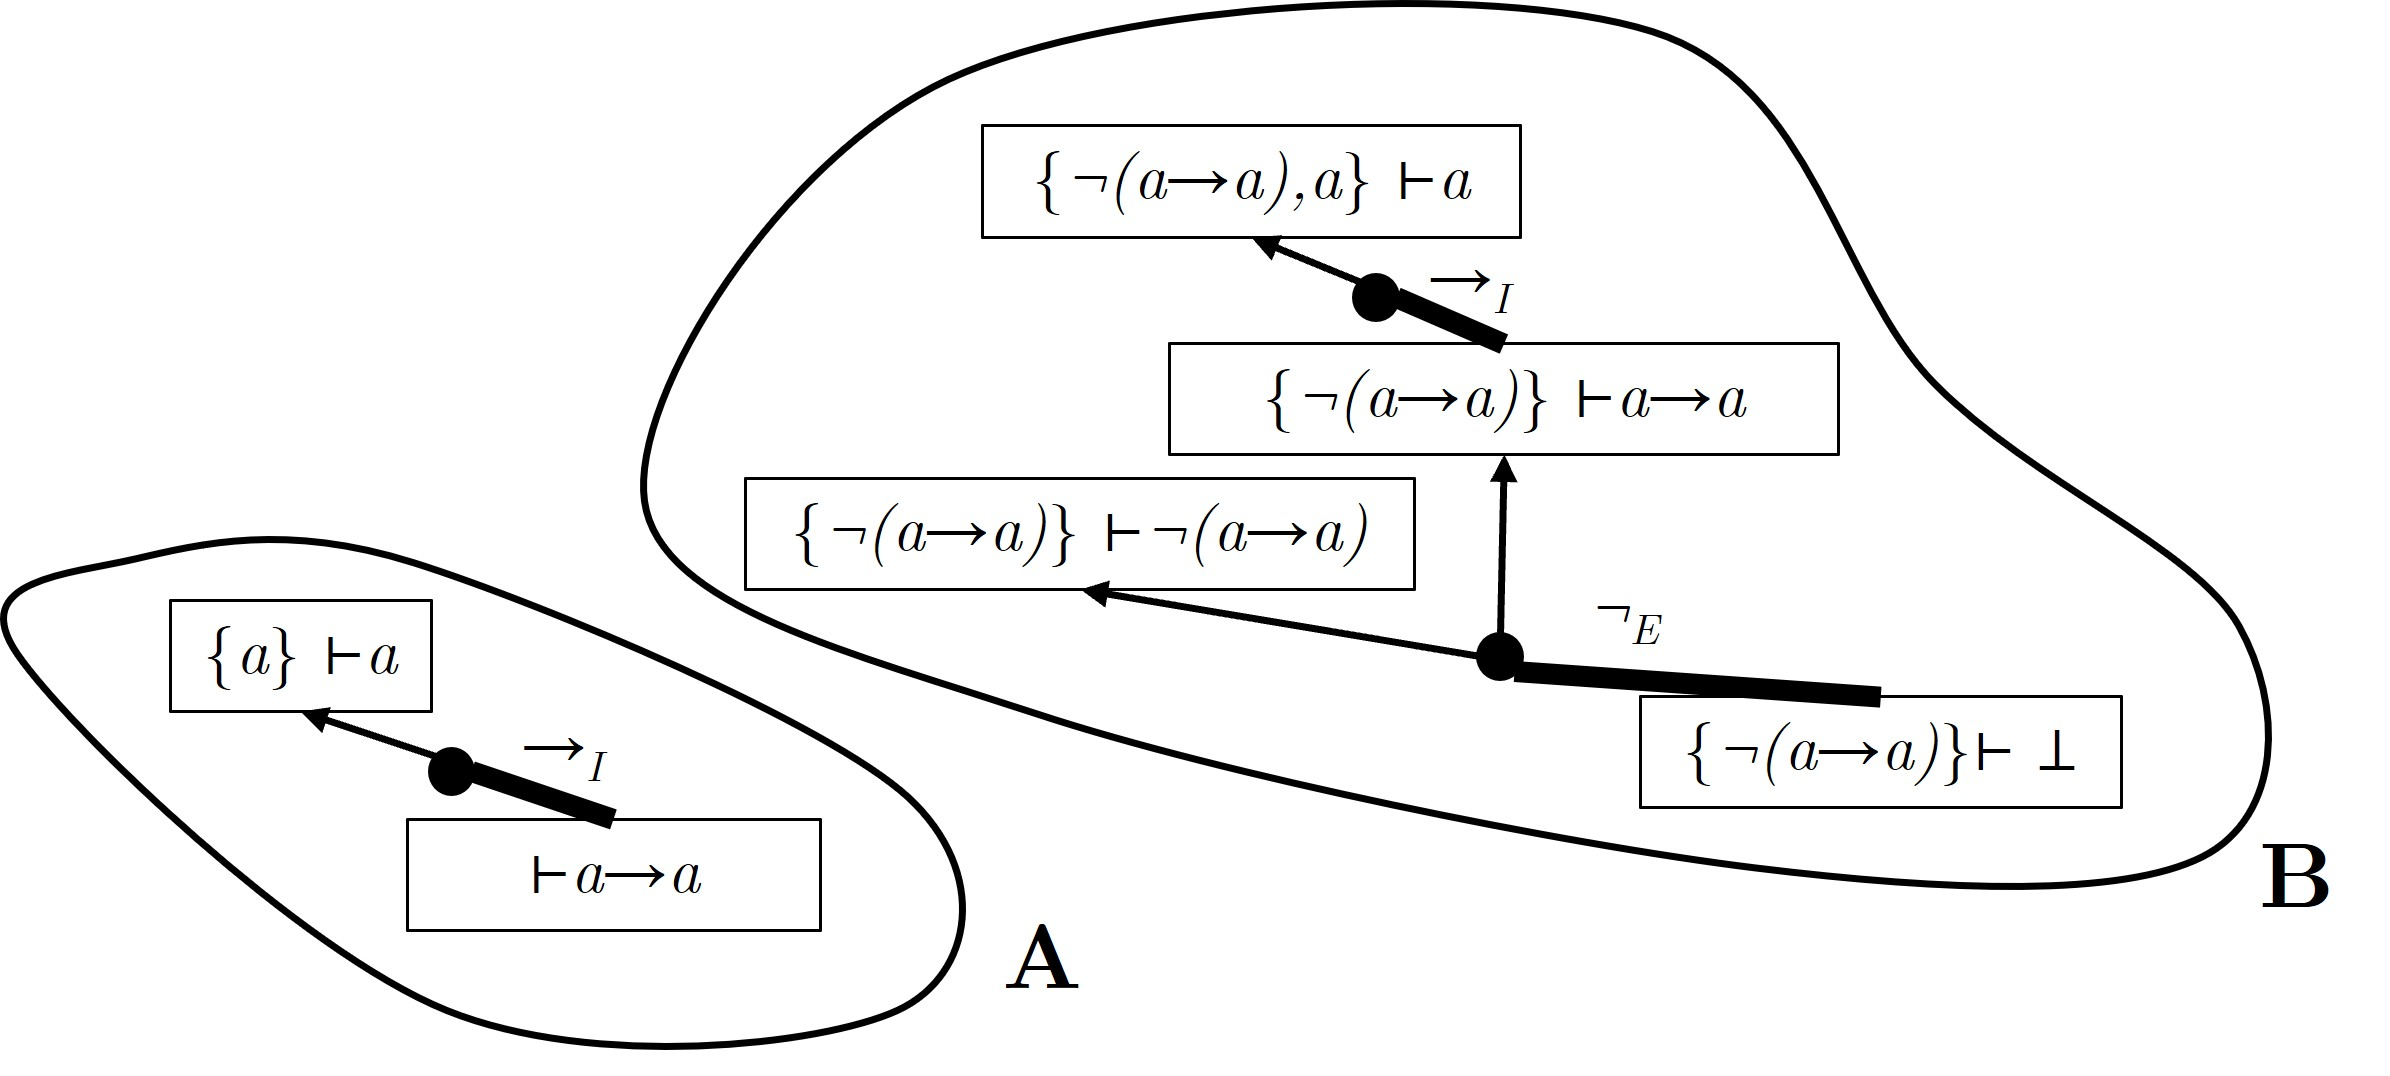
\includegraphics[width=1\linewidth]{resources/sg-final.jpg}
    \caption{Trimmed State Graph showing valid proof paths.}
    \label{fig:sg-trim}
\end{figure}

To check whether a valid solution was found for the full proof, we simply verify if the initial state appears in the trimmed graph. In the example above, the solution corresponds to tree \textbf{A}, as we want to solve the problem \(\vdash a \to a\). That solution is always the smallest in height/size, respectively. With this trimmed graph, we can now generate feedback by querying which states are still missing in the student’s proof. Figures \ref{fig:extract-solution} and \ref{fig:extract-solution2} illustrate examples of how feedback can be generated from the final graph.

In this first example, the student does not know how to proceed after applying the Absurdity rule. By running the algorithm and querying the final graph with the state that is still unsolved, we get a possible solution. This case represents tree \textbf{B} in Figure~\ref{fig:sg-trim}. Knowing the remaining part of the proof, we can generate feedback. For example, we can tell the student to apply the Elimination of the Negation rule using \(a \to a \) and  \(\lnot(a \to a) \) (\textbf{Providing guidance on rule applications}). In this specific case, we cannot give hints about sub-proofs to solve the problem, as the solution is already small. But in some cases where the solution is bigger, we can do that (\textbf{Breaking proofs into smaller sub-proofs}). We can also specify how far the student is from the final proof. In this case, we can say that they are two rules away from completing the proof (\textbf{Indicating the distance to a solution}). Finally, we can also suggest some improvements in the resolution. In this case, the student shifts their solution by applying the Absurdity rule, making it longer. That information can also be extracted from the graph by comparing the smallest proof (the one with the initial state) with the student’s final proof (\textbf{Improvements in the proof}).

 
\begin{figure}
    \centering
    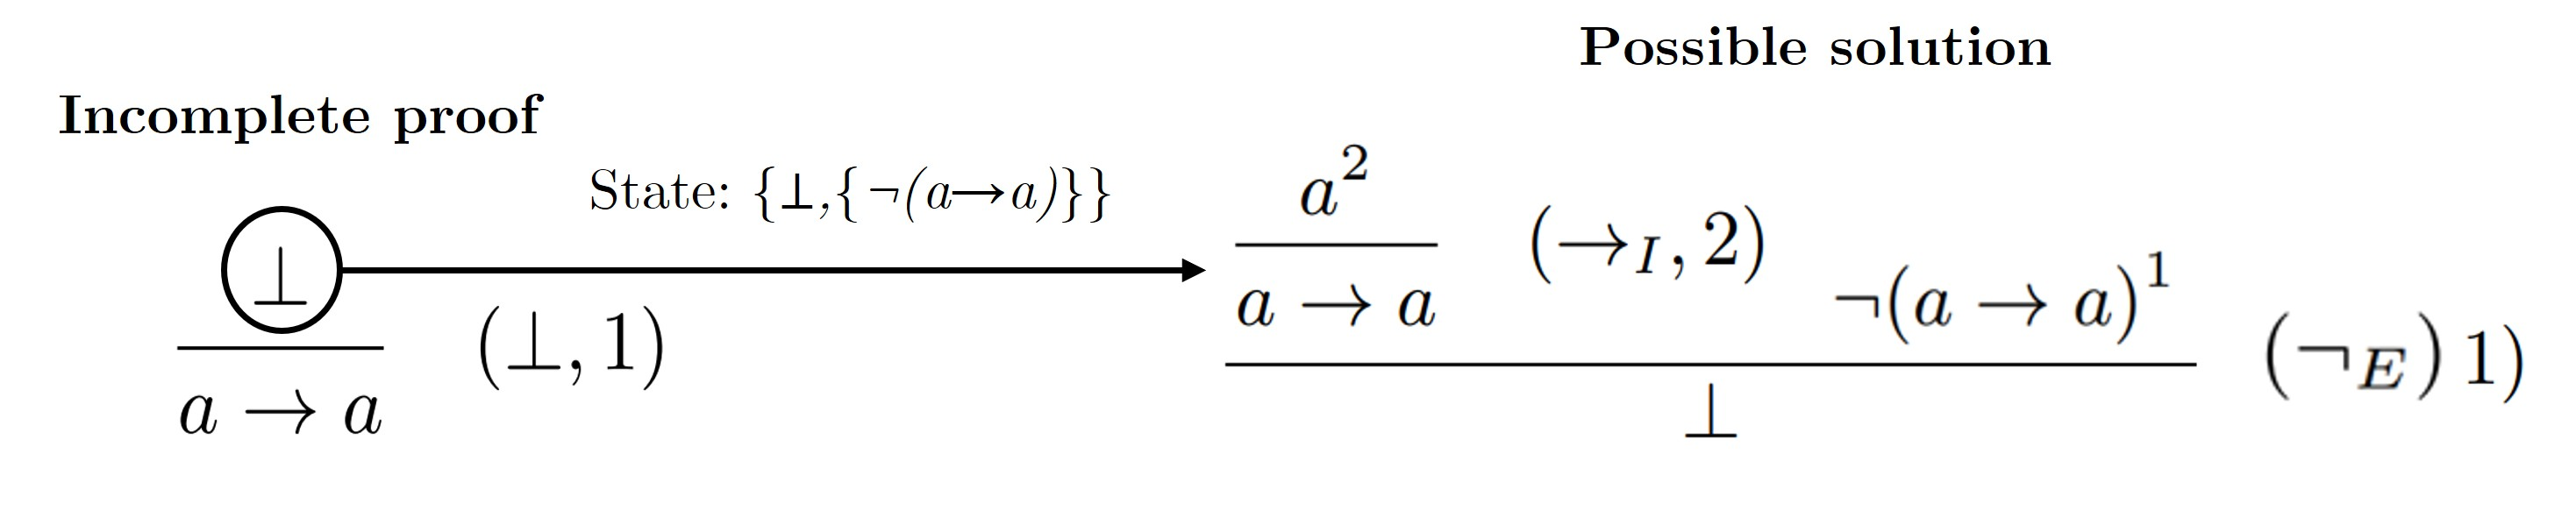
\includegraphics[width=1\linewidth]{resources/trim-pos-feed.jpg}
    \caption{Extracting a solution to produce feedback using an existing state}
    \label{fig:extract-solution}
\end{figure}

In this second example, a solution cannot be found, as the state assigned to the unresolved part of the proof does not belong to the final graph. In this case, we can inform the student that the path they are taking may be too complex, and we can suggest going back \(X\) rule applications until the algorithm finds the correct path again to guide the student. We cannot affirm that there is no solution, because we may not have explored the whole space of possible solutions. In this example, if the student removes the Elimination of Negation rule (one step back), we return to the situation previously presented.

\begin{figure}
    \centering
    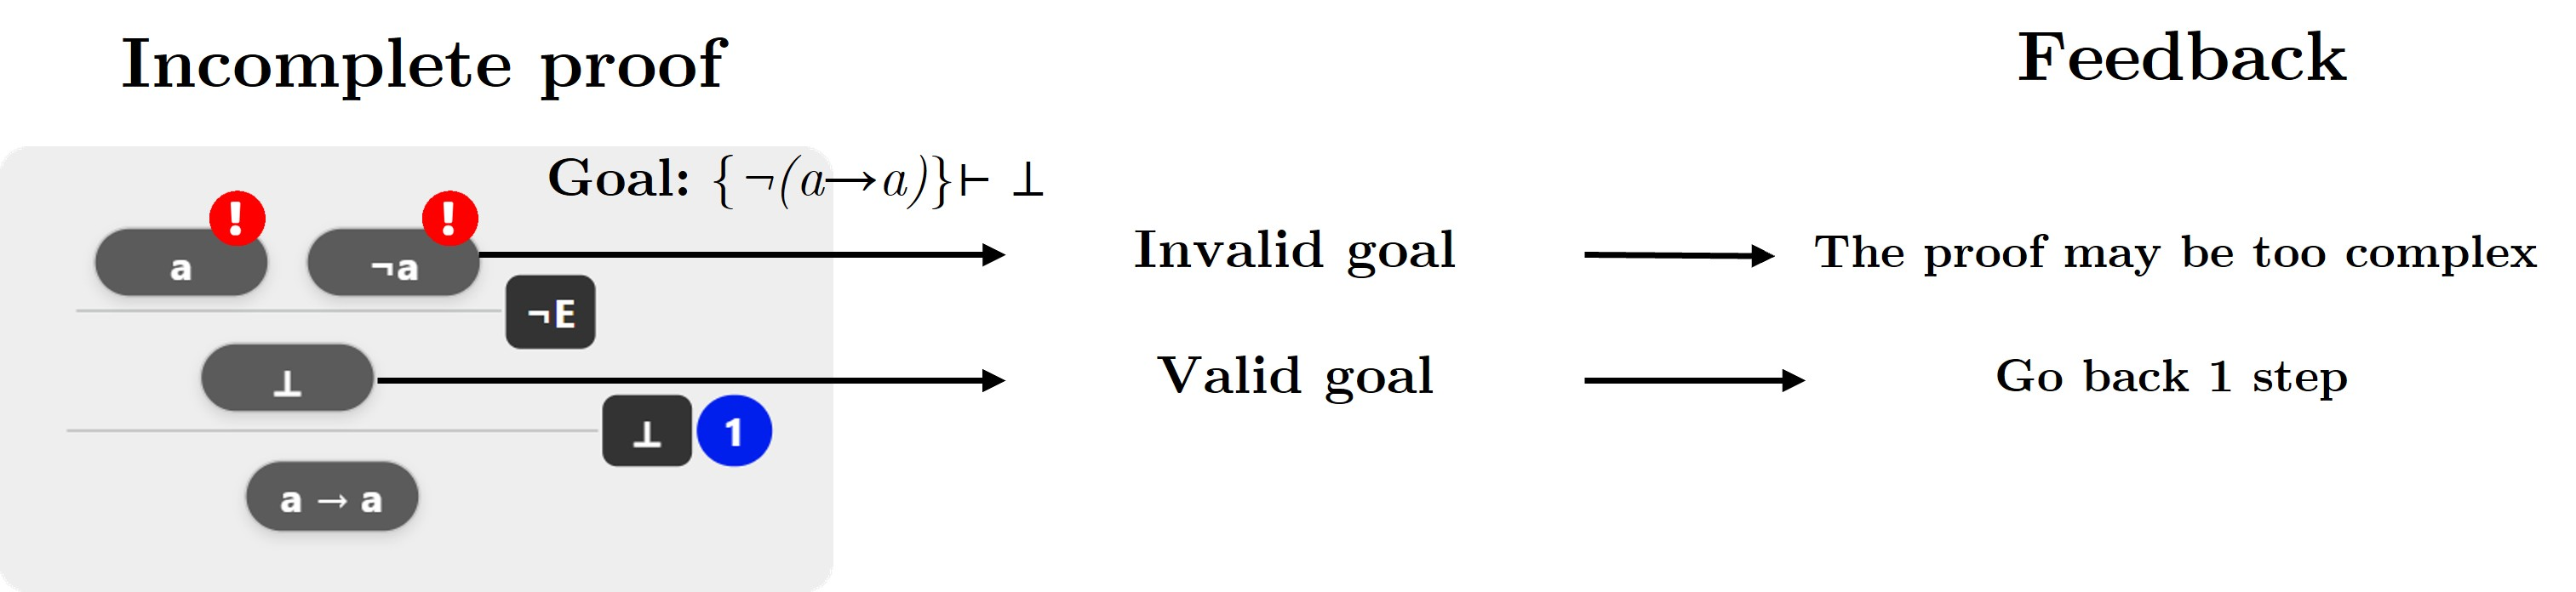
\includegraphics[width=1\linewidth]{resources/trim-neg-feed.jpg}
    \caption{Extracting a solution to produce feedback using a non-existing state.}
    \label{fig:extract-solution2}
\end{figure}

These methodologies can also be used to assess exercises. For example, by computing how far the student’s resolution is from a possible solution if the problem remains unsolvable, or how far it is shifted from the best solution. In some cases, based on the size of the explored solution space, we can say that the student overcomplicated the resolution.
